\documentclass[12pt]{article}
\usepackage{geometry}                % See geometry.pdf to learn the layout options. There are lots.
\geometry{letterpaper}                   % ... or a4paper or a5paper or ... 
\usepackage{graphicx}
\usepackage{amssymb}
\usepackage{amsthm}
\usepackage{epstopdf}
\usepackage[english, german]{babel}
\usepackage[utf8]{inputenc}
\usepackage[usenames,dvipsnames]{color}
\usepackage[table]{xcolor}
\usepackage{hyperref}
\DeclareGraphicsRule{.tif}{png}{.png}{`convert #1 `dirname #1`/`basename #1 .tif`.png}

\theoremstyle{definition}
\newtheorem{example}{Example}

\newenvironment{explanation}{%
   \setlength{\parindent}{0pt}
   \itshape
   \color{blue}
   \normalfont
}{}

\newcommand{\projectname}{Dahoam}
\newcommand{\productname}{Dahoam}
\newcommand{\projectleader}{I. Gattringer}
\newcommand{\documentstatus}{In process}
%\newcommand{\documentstatus}{Submitted}
%\newcommand{\documentstatus}{Released}
\newcommand{\version}{V. 1.0}

\begin{document}
\begin{titlepage}
\begin{flushright}

\includegraphics[scale=.5]{htlleondinglogo.png}\\
\end{flushright}

\vspace{10em}

\begin{center}
{\Huge System Specification} \\[3em]
{\LARGE \productname} \\[3em]
\end{center}

\begin{flushleft}
\begin{tabular}{|l|l|}
\hline
Project Name & \projectname \\ \hline
Project Leader & \projectleader \\ \hline
Document state & \documentstatus \\ \hline
Version & \version \\ \hline
\end{tabular}
\end{flushleft}

\end{titlepage}
\section*{Revisions}
\begin{tabular}{|l|l|l|}
\hline
\cellcolor[gray]{0.5}\textcolor{white}{Date} & \cellcolor[gray]{0.5}\textcolor{white}{Author} & \cellcolor[gray]{0.5}\textcolor{white}{Change} \\ \hline
November 03, 2019&P. Bauer&First version \\ \hline
\end{tabular}
\pagebreak

\tableofcontents
\pagebreak

\section{Initial Situation and Goal}  
\subsection{Initial Situation}
An initial prototype of Dahoam was built between 2018 and 2019. It combines a commercial mirror with a smart home hub.
The mirror is capable of:
\begin{itemize}
    \item recognizing when a person stands in front of it. If the person is unknown, they can register themselves through Dahoam-Connect-App.
    \item understanding when the user is speaking to him (only with a predefined word pool.
    \item showing weather data of a static location.
    \item adding an email address via POP3 to a user account.
    \item adding a calendar to a user account and showing upcoming events on the mirror.
    \item speaking to the user after commands with a predefined word pool.
    \item integrating static MQTT smart home interfaces (temperature sensor and light)
\end{itemize}
\\
The reasons for carrying out the project was to enhance the mirror in all aspects and create a smart mirror which is practically useful. It is in interest of the headmaster and head of department of HTL Leonding to have a project like Dahoam which represents most of the technical focuses of the school.

\subsubsection{Application Domain}
Dahoam operates with 5 microservices. Face recognition spots a person in front of the mirror and compares it to all known user. When the person is already registered, they will be logged into the mirror. If the person is unknown to the mirror, they can register them. While registration and other processes, interaction is done through voice commands. The mirror understands spoken words via speech recognition, which sends the understood words to the third microservice, the intent parser. It tries to find out what the intention of the user is and sends the intent to the master service. The master service stands in between all services and handles the whole system. 
For confirmation after startup of the mirror or successfully done tasks the mirror gives feedback to the user through speaking to them via Text-To-Speech service.\\
Each user can operate their own account where they can also add a specific email address via POP3 and a calendar. The user is able to log in on the mirror with just standing in front of the camera or into the Dahoam-Connect-App with their nickname and password. Managing their account is only possible in the app.
\\
Smart home interfaces are added statically. Sensor values can be requested from the user via speech interaction directly with the mirror. Same goes for turning on/off the lights.

\subsubsection{Glossary}

\begin{flushleft}
\begin{tabular}{|l|l|}
\hline
Text-To-Speech & Converts output to spoken words\\ \hline
Speech Recognition & Converts spoken input to text\\ \hline
Intent Parser & Parses input to executable commands\\ \hline
Face Recognition & Compares faces in front of the camera with saved faces\\ \hline
Master Service & Interface of all other services\\ \hline
Dahoam-Connect-App & Smartphone app for user/mirror configurations\\ \hline
\end{tabular}
\end{flushleft} 
\subsubsection{Model of the Application Domain}
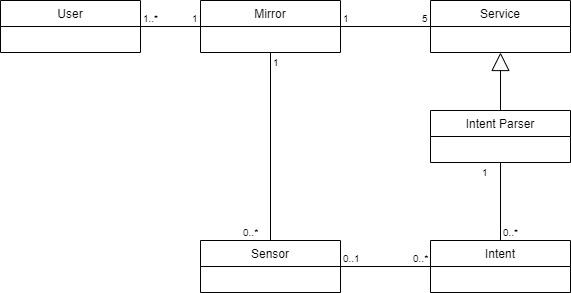
\includegraphics[scale=.6]{ClassDiagram.png}

\pagebreak
\subsection{Goal}

Dahoam should give the customer a solid smart home hub integrated in a common mirror. The intelligent mirror will run 24/7 and is only active when a person is in front of it. If there is one, a movement sensor will wake up all services. By switching into a sleep mode, the power consumption is reduced. \\
When starting the mirror the first time, the user has to connect to the hot spot from Dahoam. When connecting to the network, a website will open where the user has to enter an admin account and enter the mirror location for weather information.
An advanced Dahoam-Connect-App has following additional features:
\begin{itemize}
    \item Integration of new smart home gadgets
    \item Configuration of an individual weather location for each user
    \item Adding an email account for each user via IMAP
    \item Deleting users
    \item Admin role page where general mirror configuration can be done
\end{itemize}

\pagebreak

\section{Functional Requirements}
\subsection{Overview}
\begin{center}
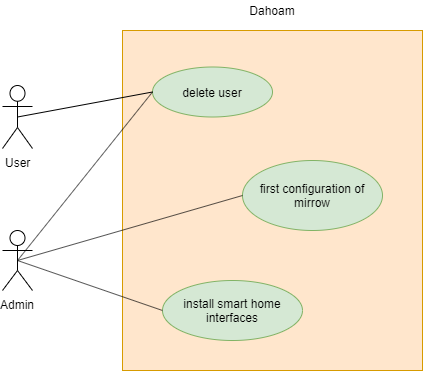
\includegraphics[scale=.7]{UseCase/UseCase.png}\\
\end{center}

\subsection{Use Case 1: Delete User}
\subsubsection{General Description}
In the user settings exists a ``delete'' button which deletes all related user data.
\\
\\
\begin{tabular}{|p{.2\linewidth}|p{.65\linewidth}|}
\hline 
ID: & Delete User/Admin \\ \hline
Goal: & The user wants to be able to delete their own account. \\ \hline
Precondition: & The use case will be triggered by pressing the ``delete'' button in the Dahoam-Connect-App. \\ \hline
Postcondition: & The user is deleted and will not be recognized by the mirror anymore. Also the user will not be able to log in with the deleted account in the app. \\ \hline
Involved Users: & Role name: user, admin  \\ \hline
\end{tabular}

\subsubsection{UI to Call the Use Case}
This is the design of the user settings, where the delete button will be added. With this button it will be possible to delete the account logged in.

\begin{center}
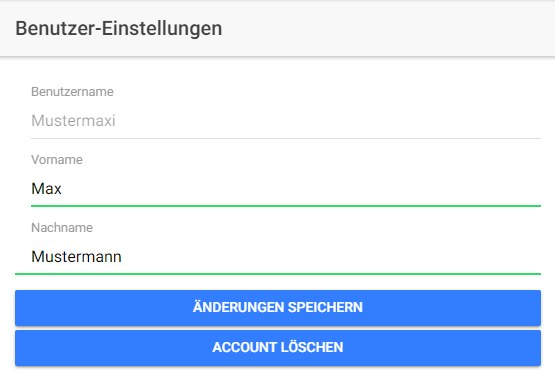
\includegraphics[scale=.8]{UseCase/DeleteUserFirstStep.PNG}\\
\end{center}
\subsubsection{The Standard Use}
The user clicks the button and their account will be deleted. The app will automatically log out the account and the mirror does not recognize the user again.\\\\
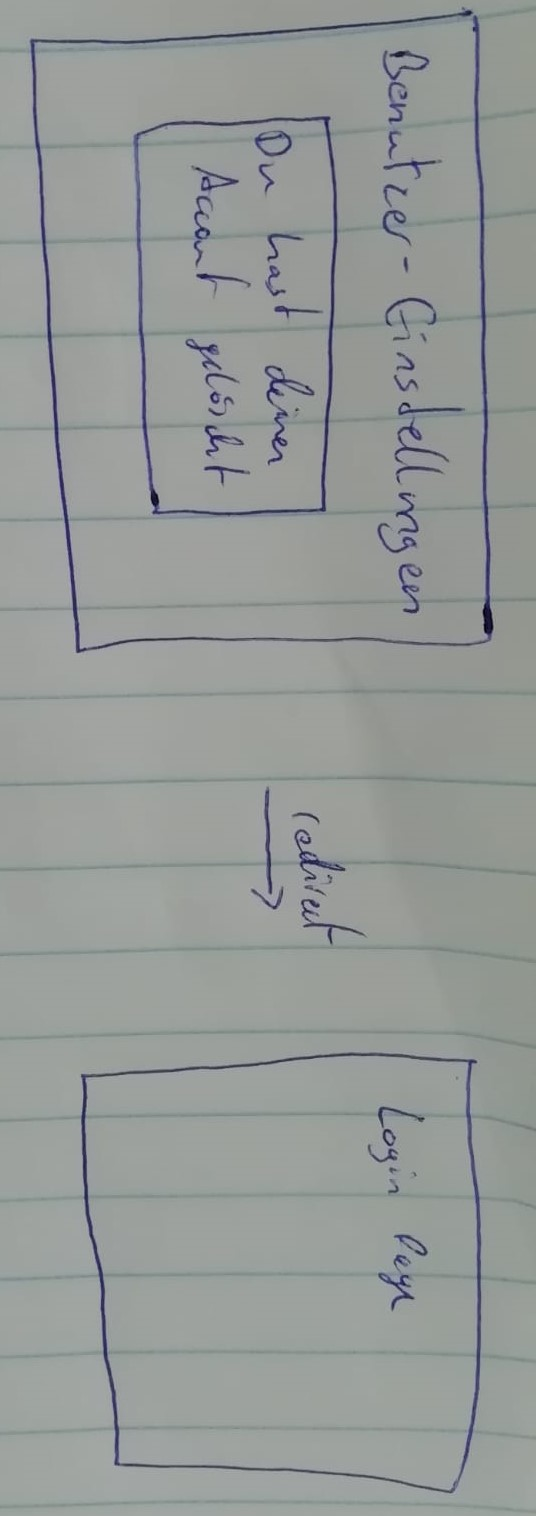
\includegraphics[angle=90, scale=.3]{UseCase/UIDELETEUSER2.png}\\

\subsubsection{The Non-Standard Use}
If the last admin of the mirror wants to delete their account, an error message must occur, because without an admin, the mirror can not change the smart home interfaces.\\\\
 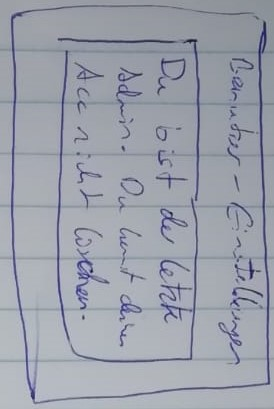
\includegraphics[angle=90, scale=.5]{UseCase/LetzterAdminWillAccountLoschen.jpeg}\\

\subsection{Use Case 2: First Configuration of the Mirror}
\subsubsection{General Description}
The user has to connect to the hot spot which the mirror provides. Then a website will be opened on the gadget from which the user connected to the hot spot. There the mirror can be connected to the actual network and define its location.\\
After this, the problem of having a non-static IP still exists. Therefore it is recommended to give the mirror a static IP. This also it makes it a lot easier for the Dahoam-Connect-App to handle.\\\\
\begin{tabular}{|p{.2\linewidth}|p{.65\linewidth}|}
\hline 
ID: & First configuration of mirror \\ \hline
Goal: & After the mirror has been installed, it must be configured, so that the mirror knows in which network it works and what its location is.\\ \hline
Precondition: & The mirror has to be built together and started for the first time.\\ \hline
Postcondition: & The mirror knows in which network it has to operate and where it is located.\\ \hline
Involved Users: & Role name: admin \\ \hline
\end{tabular}

\subsubsection{UI to Call the Use Case}
\begin{center}
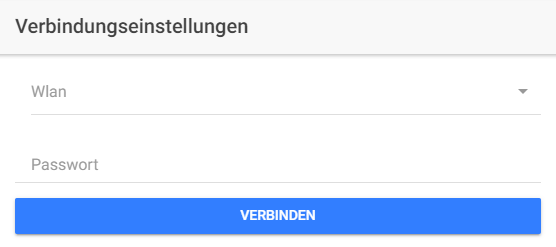
\includegraphics[scale=.8]{UseCase/StandartWlanEinstellungen.PNG}\\
\end{center}

\subsubsection{The Standard Use}
A WiFi is found and the correct password was submitted.\\\\
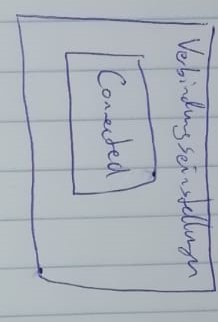
\includegraphics[angle=90, scale=.8]{UseCase/VerbindungHergestelltMitInternet.jpeg}\\\\
\\
Then the location of the mirror has to be entered. By entering a letter, a drop down list will give options for existing locations.\\\\
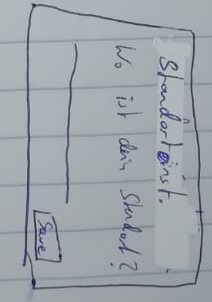
\includegraphics[angle=90, scale=.8]{UseCase/Standorteingabe.jpeg}\\\\
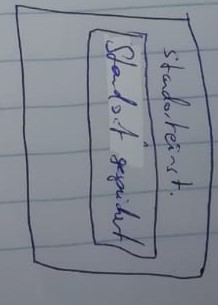
\includegraphics[angle=90, scale=.8]{UseCase/StandortGespeichert.jpeg}\\\\

\subsubsection{The Non-Standard Use}
If there is no WiFi to connect to, the mirror cannot fulfill its main purpose - being a smart home hub.
Therefore an error message will be shown to the user. Also he will not be able to continue the process of configuring the mirror until it is connected to a WiFi.\\
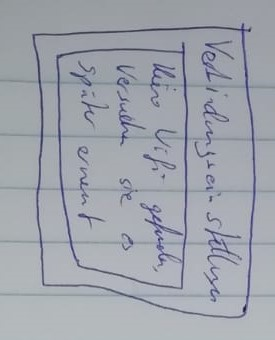
\includegraphics[angle=90, scale=.8]{UseCase/KeinWifiGefunden.jpeg}\\\\
If a WiFi got selected, but the user entered a wrong password, an alert will appear to communicate this to the user.\\\\
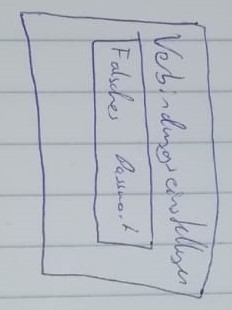
\includegraphics[angle=90, scale=.8]{UseCase/VerbindungFalschesPasswort.jpeg}\\


\subsection{Use Case 3: Install Smart Home Interfaces}
\subsubsection{General Description}
Connecting Smart Home Devices to the mirror with the help of MQTT. \\
\\
\begin{tabular}{|p{.2\linewidth}|p{.65\linewidth}|}
\hline 
ID: & Install smart home interfaces\\ \hline
Goal: & Connecting the mirror with smart home devices.\\ \hline
Precondition: & Admin presses the button for installing the interfaces.\\ \hline
Postcondition: & The mirror knows all different smart home devices which are installed. \\ \hline
Involved Users: & Role name: admin  \\ \hline
\end{tabular}

\subsubsection{UI to Call the Use Case}
\begin{center}
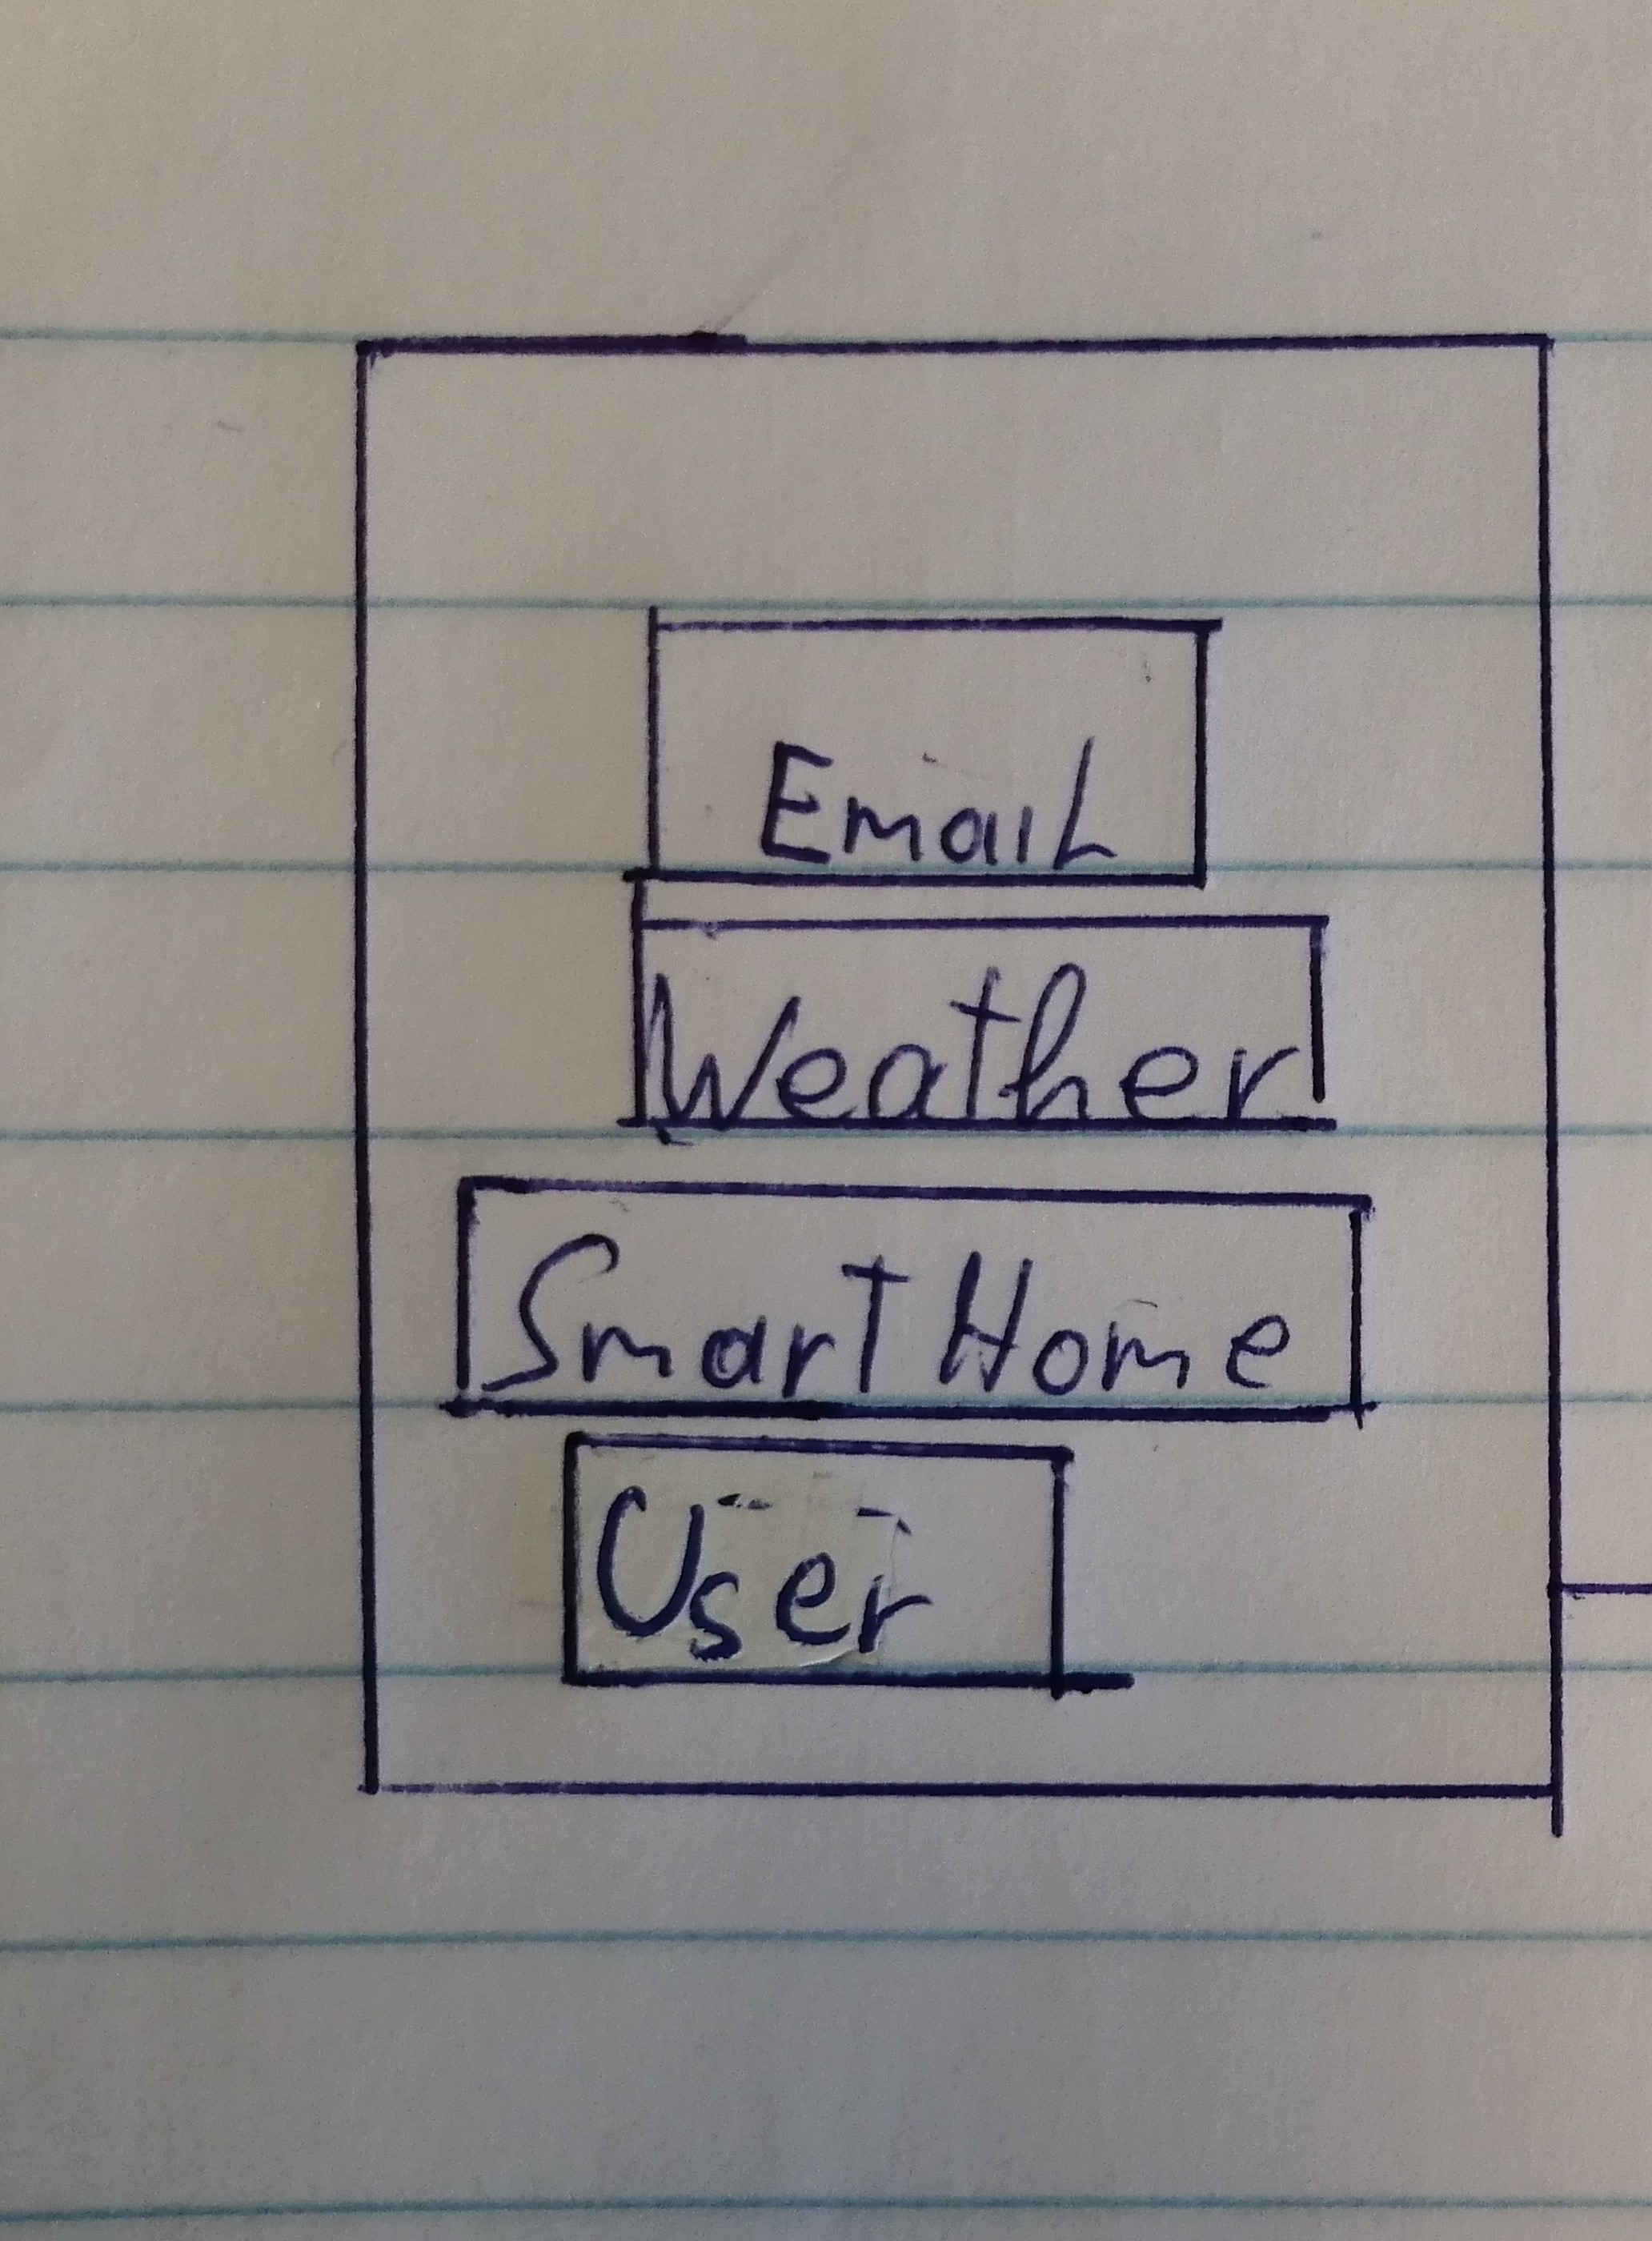
\includegraphics[scale=.1]{UseCase/StandardView.jpg}\\
\end{center}

\subsubsection{The Standard Use}
First, a MQTT broker has to be set in the Dahoam-Connect-App. After pressing the connect button a small alert will be displayed. When connected, devices can be added. First a list of all existing devices will be shown with an add button at the bottom. When a publication is added, it is needed to specify a name as well as the topic. QoS and retained are optional. To finish the procedure it is necessary to select, which type of values will be sent. Subscription is more or less the same, but there has to be set the name and topic, since data will be received.\\

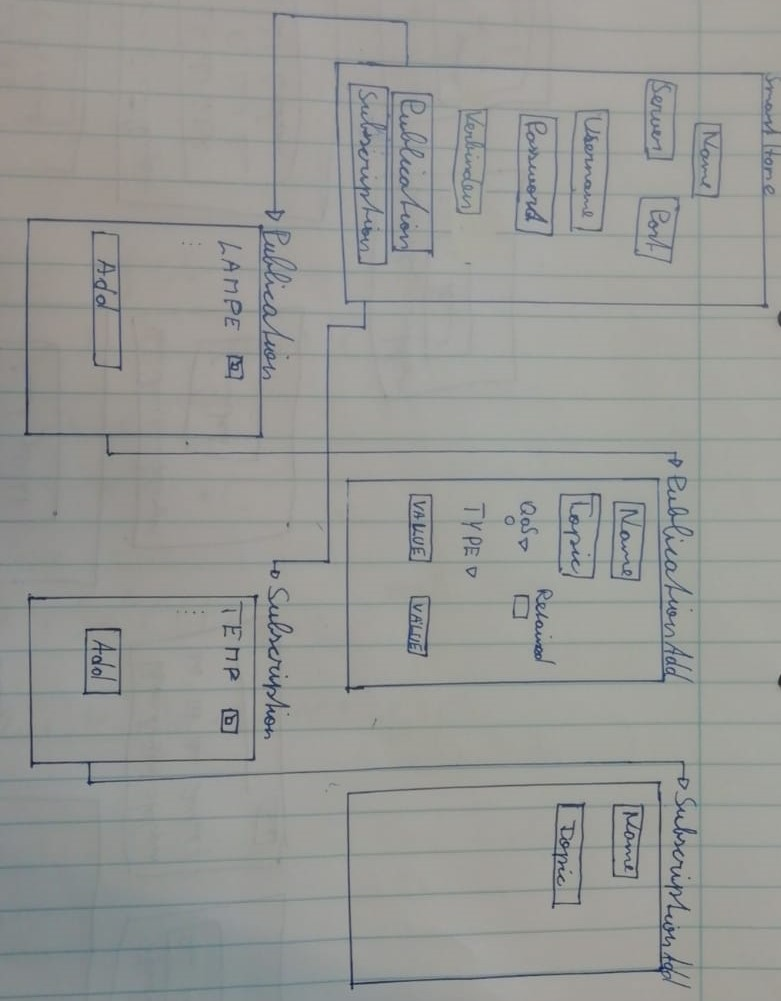
\includegraphics[angle=90, scale=.5]{UseCase/InstallSmartHomeInterfaces.jpeg}\\

\subsubsection{The Non-Standard Use}
When the user does not enter the right credentials for the broker, an alert occurs and warns him.


\subsection{Use Case 4: User Administration}
\subsubsection{General Description}
Admin accounts are able to administrate users. By clicking the user button, a list of all users in the system appears.\\
\\
\begin{tabular}{|p{.2\linewidth}|p{.65\linewidth}|}
\hline 
ID: & User administration\\ \hline
Goal: & The admin should be able to see a list of all users and be able to delete users that are not marked as admin. It is also possible to give another user admin rights.\\ \hline
Precondition: & The admin clicks the user button to get all users.\\ \hline
Postcondition: & A User has been deleted or has gotten admin rights.\\ \hline
Involved Users: & Role name: admin  \\ \hline
\end{tabular}

\subsubsection{UI to Call the Use Case}
\begin{center}
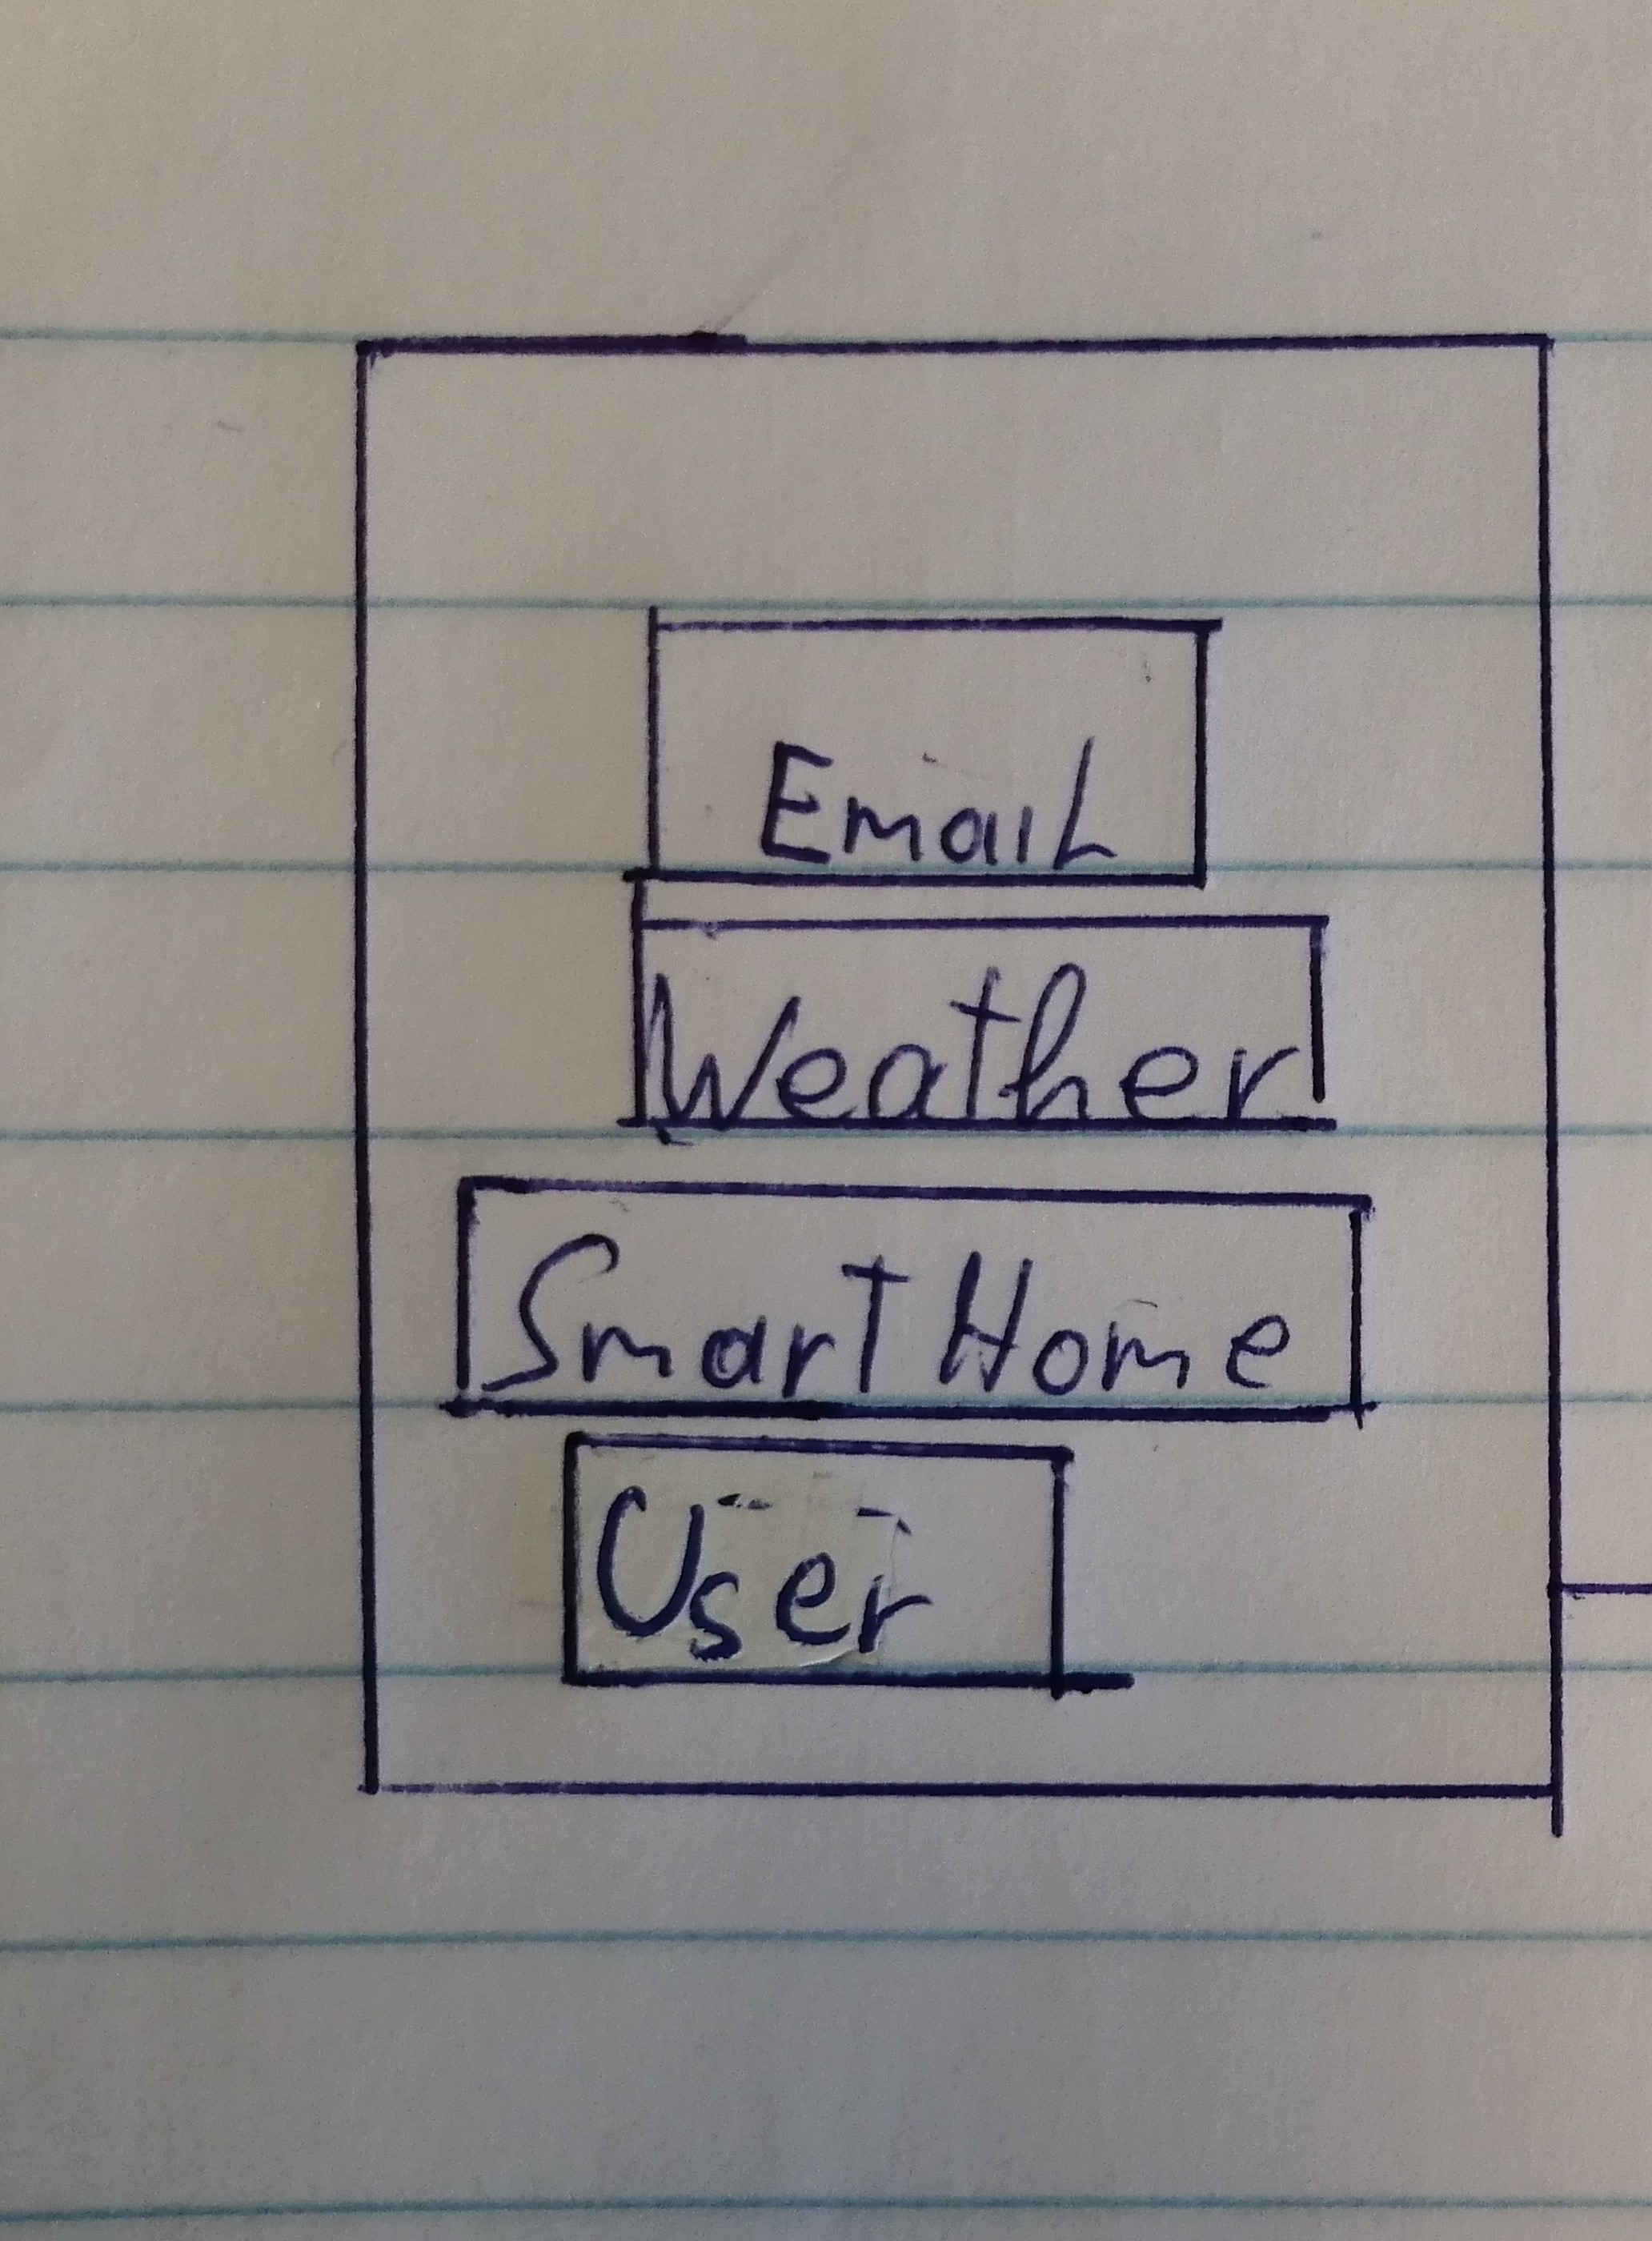
\includegraphics[scale=.1]{UseCase/StandardView.jpg}\\
\end{center}

\subsubsection{The Standard Use}
\begin{itemize}
    \item Users can be deleted by a admin as long as it is not an admin account.
    \item Admins can give other users admin rights.
\end{itemize}
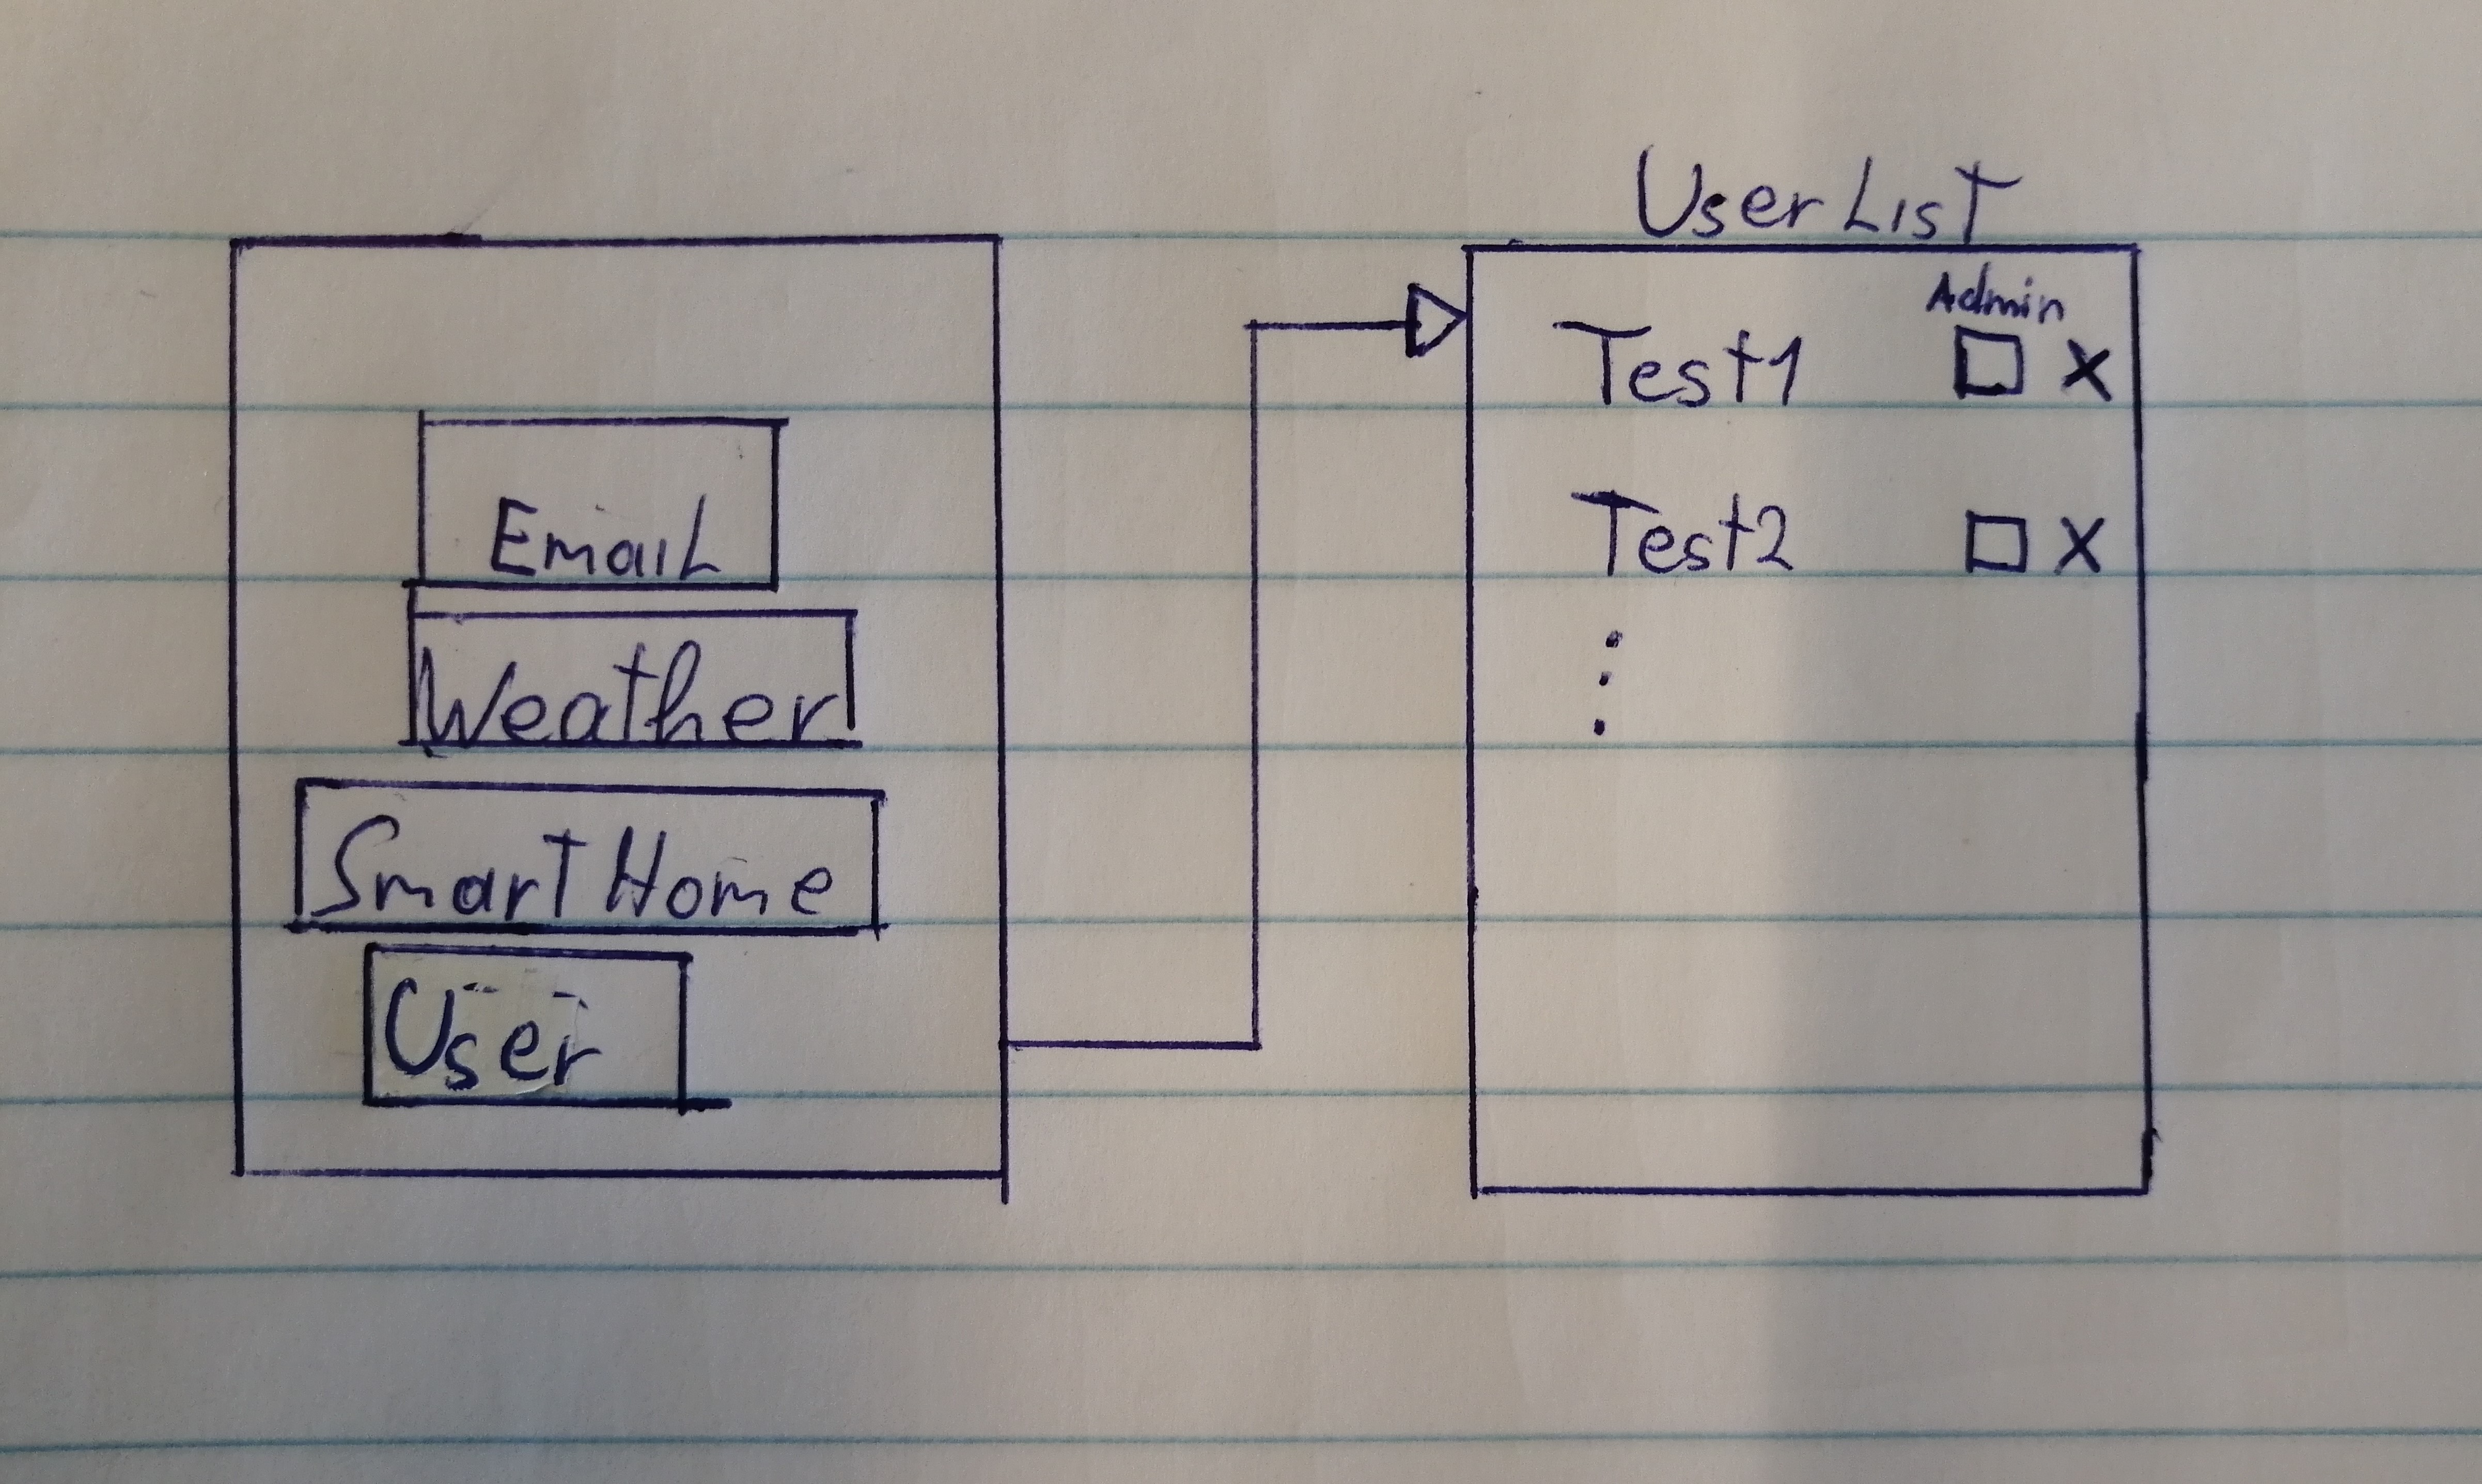
\includegraphics[scale=.1]{UseCase/UserAdministration.jpg}\\

\subsubsection{The Non-Standard Use}
\begin{itemize}
    \item Admins can not delete other admins. If they try, an error  will occur.  
\end{itemize}

\subsection{Use Case 5: Sleep Mode}
\subsubsection{General Description}
When the mirror does not detect any movement for a certain amount of time it enters the sleep mode to save energy. \\

\begin{tabular}{|p{.2\linewidth}|p{.65\linewidth}|}
\hline 
ID: & Sleep mode\\ \hline
Goal: & The mirror does use a lot less energy and does not heat up to fast.\\ \hline
Precondition: & The mirror is running. \\ \hline
Postcondition: & The mirror is in sleep mode. \\ \hline
Involved Users: & Role name: user \\ \hline
\end{tabular}

\subsubsection{The Standard Use}
The mirror is in the sleep mode whenever no one has used it recently and waits for a user to move in front of it. This is important to do something against the overheating problem. For sleeping mode unused services will be stopped.

\subsubsection{The Non-Standard Use}
The mirror does not enter the sleep mode correctly or never enters it.

\subsection{Use Case 6: Wake up from Sleep Mode}
\subsubsection{General Description}

\begin{tabular}{|p{.2\linewidth}|p{.65\linewidth}|}
\hline 
ID: & Wake up from sleep mode\\ \hline
Goal: & When user stands in front of the mirror, it ``wakes up''.\\ \hline
Precondition: & Mirror is in sleep mode and user stands in front of the mirror.\\ \hline
Postcondition: &  Mirror is running. \\ \hline
Involved Users: & Role name: user \\ \hline
\end{tabular}

\subsubsection{The Standard Use}
The mirror recognizes movement via a motion sensor and wakes up from sleep mode. After this, the user is able to use the mirror. All stopped services start again.

\subsubsection{The Non-Standard Use}
\begin{itemize}
    \item The motion sensor does not detect any movement, despite a user standing in front of it.
    \item One of the stopped containers got unhealthy and cannot be started anymore.
\end{itemize}


\subsection{Use Case 7: Creating First Admin}
\subsubsection{General Description}
The first user that registers himself, will automatically be an admin.\\

\begin{tabular}{|p{.2\linewidth}|p{.65\linewidth}|}
\hline 
ID: & First admin account creation\\ \hline
Goal: & After set up an admin account exists.\\ \hline
Precondition: & No user is registered.\\ \hline
Postcondition: &  One user exists which is an admin. \\ \hline
Involved Users: & Role name: admin \\ \hline
\end{tabular}

\subsection{Use Case 8: Defining Personal Location}
\subsubsection{General Description}
When a user registers, the mirror sets their location. This is used for the weather forecast of that particular user.\\

\begin{tabular}{|p{.2\linewidth}|p{.65\linewidth}|}
\hline 
ID: & Defining personal location\\ \hline
Goal: & The weather for the selected location of the user is displayed instead of the default mirror location.\\ \hline
Precondition: & The mirror displays the default location.\\ \hline
Postcondition: &  Personal location is set instead of the default location. \\ \hline
Involved Users: & Role name: user \\ \hline
\end{tabular}

\subsubsection{The Standard Use}
The user changes the default location to their personal location in the user settings.
The weather forecast for the personal location will be displayed. \\\\
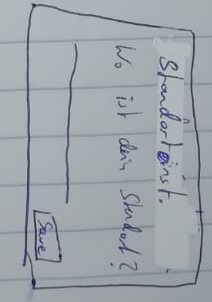
\includegraphics[angle=90,scale=.8]{UseCase/Standorteingabe.jpeg}\\
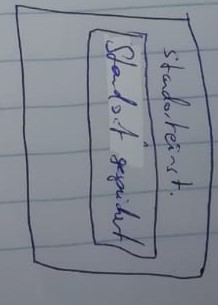
\includegraphics[angle=90,scale=.8]{UseCase/StandortGespeichert.jpeg}\\

\subsubsection{The Non-Standard Use}
The wished location could not be found or does not have a weather forecast which can be displayed at the moment.

\subsection{Use Case 9: Registration Flow}
\subsubsection{General Description}
\begin{tabular}{|p{.2\linewidth}|p{.65\linewidth}|}
\hline 
ID: & Registration flow\\ \hline
Goal: & It is easier for the user to register.\\ \hline
Precondition: & Unregistered user wants to register and stands in front of the mirror.\\ \hline
Postcondition: &  Unregistered user is registered and gets recognized by the mirror with the face recognition. \\ \hline
Involved Users: & Role name: user \\ \hline
\end{tabular}

\subsubsection{The Standard Use}
The user says the keyword ``register'', so that the mirror knows that the user wants to register. Then a window appears, which tells the user to position correctly in front of the mirror.\\\\


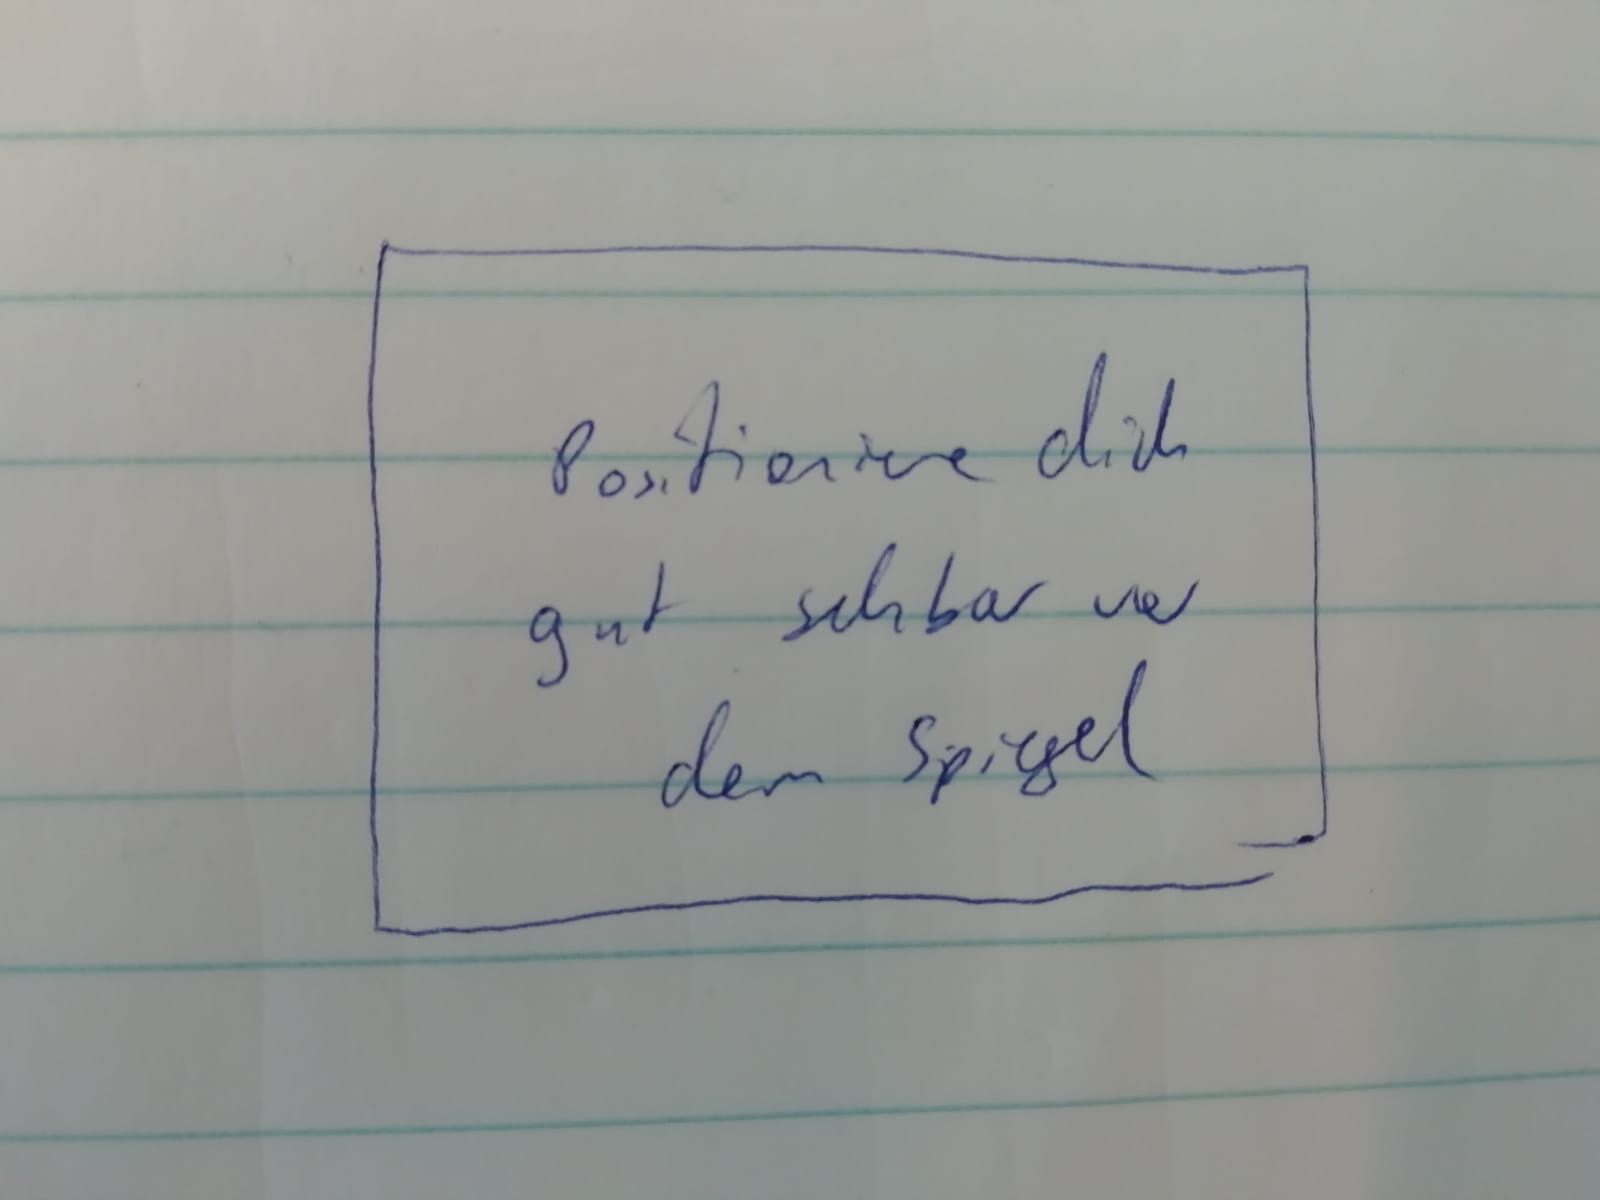
\includegraphics[scale=.1]{UseCase/PositionCorerectlyRegistrationAlert.jpeg}\\
After the message, a live broadcast of the  mirror's camera appears and the user has 5 seconds to prepare for taking a picture. \\
\\
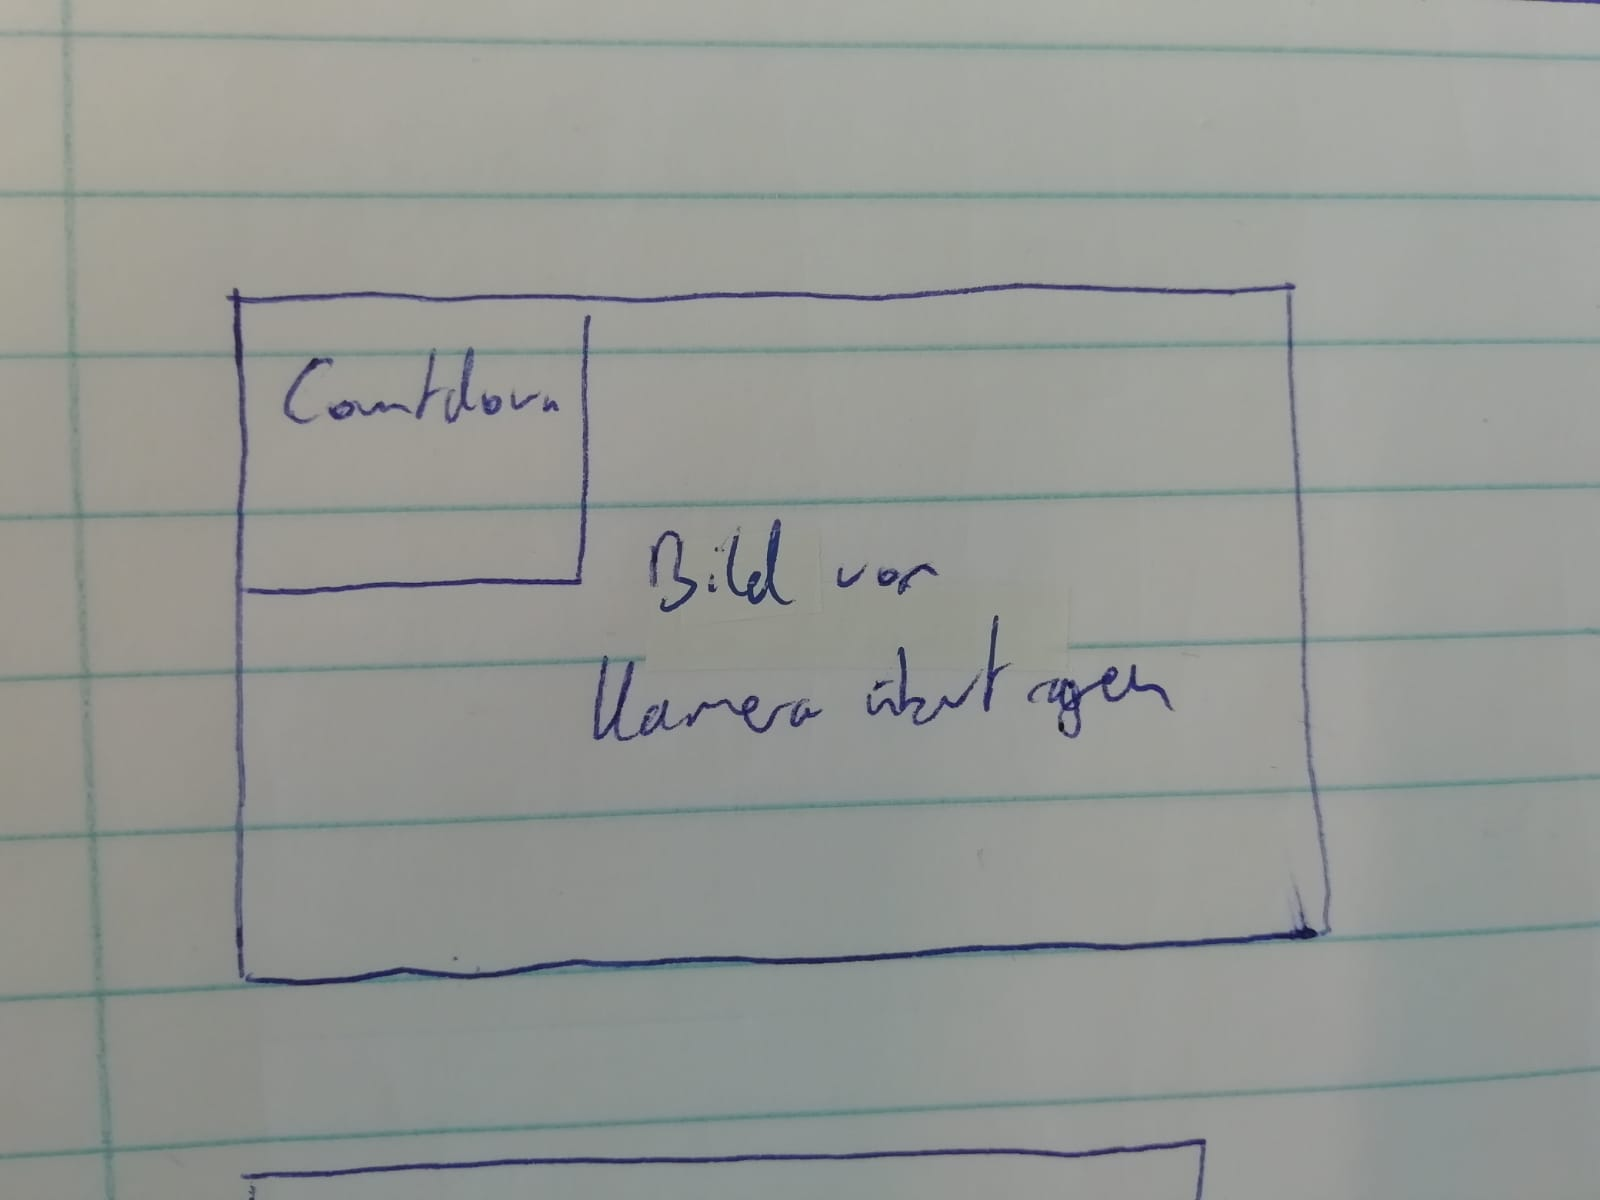
\includegraphics[scale=.1]{UseCase/RegistrationCountdownLiveBild.jpeg}\\
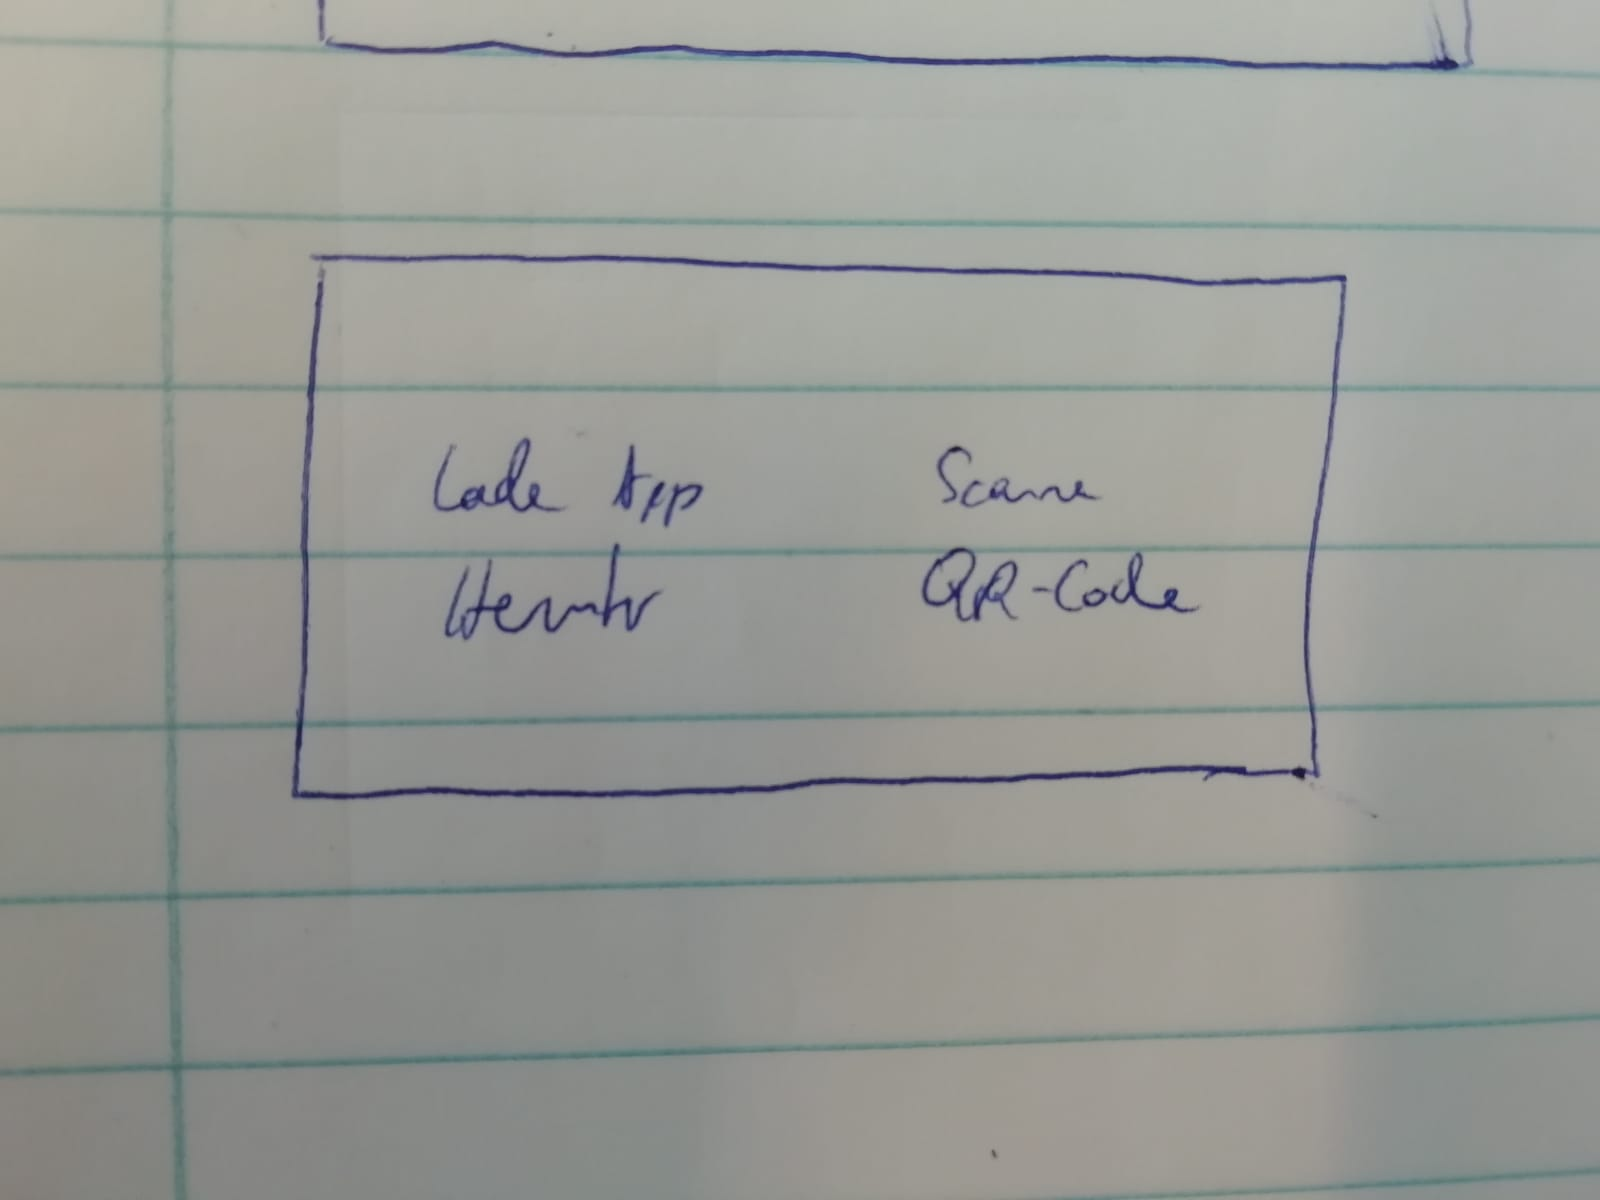
\includegraphics[scale=.1]{UseCase/DownloadDahoamAppAndScanQR-CodeREgistration.jpeg}\\
After this step, the user has to connect the Dahoam-Connect-App to the mirror by either scanning the qr-code with the App or using the alternative. Then the user has to enter their credentials. 

\subsubsection{Registration aborted by timeout}
If the user does not finish the registration process within 5 minutes, the registration will be aborted and the taken picture and information will be deleted.

\subsubsection{Registration aborted by user}
The user is able to abort the registration by saying ``abbrechen'' or pressing the button ``abbrechen'' on the Dahoam-Connect App. After aborting the taken picture and information will be deleted.\\

\subsubsection{Activity Diagram}
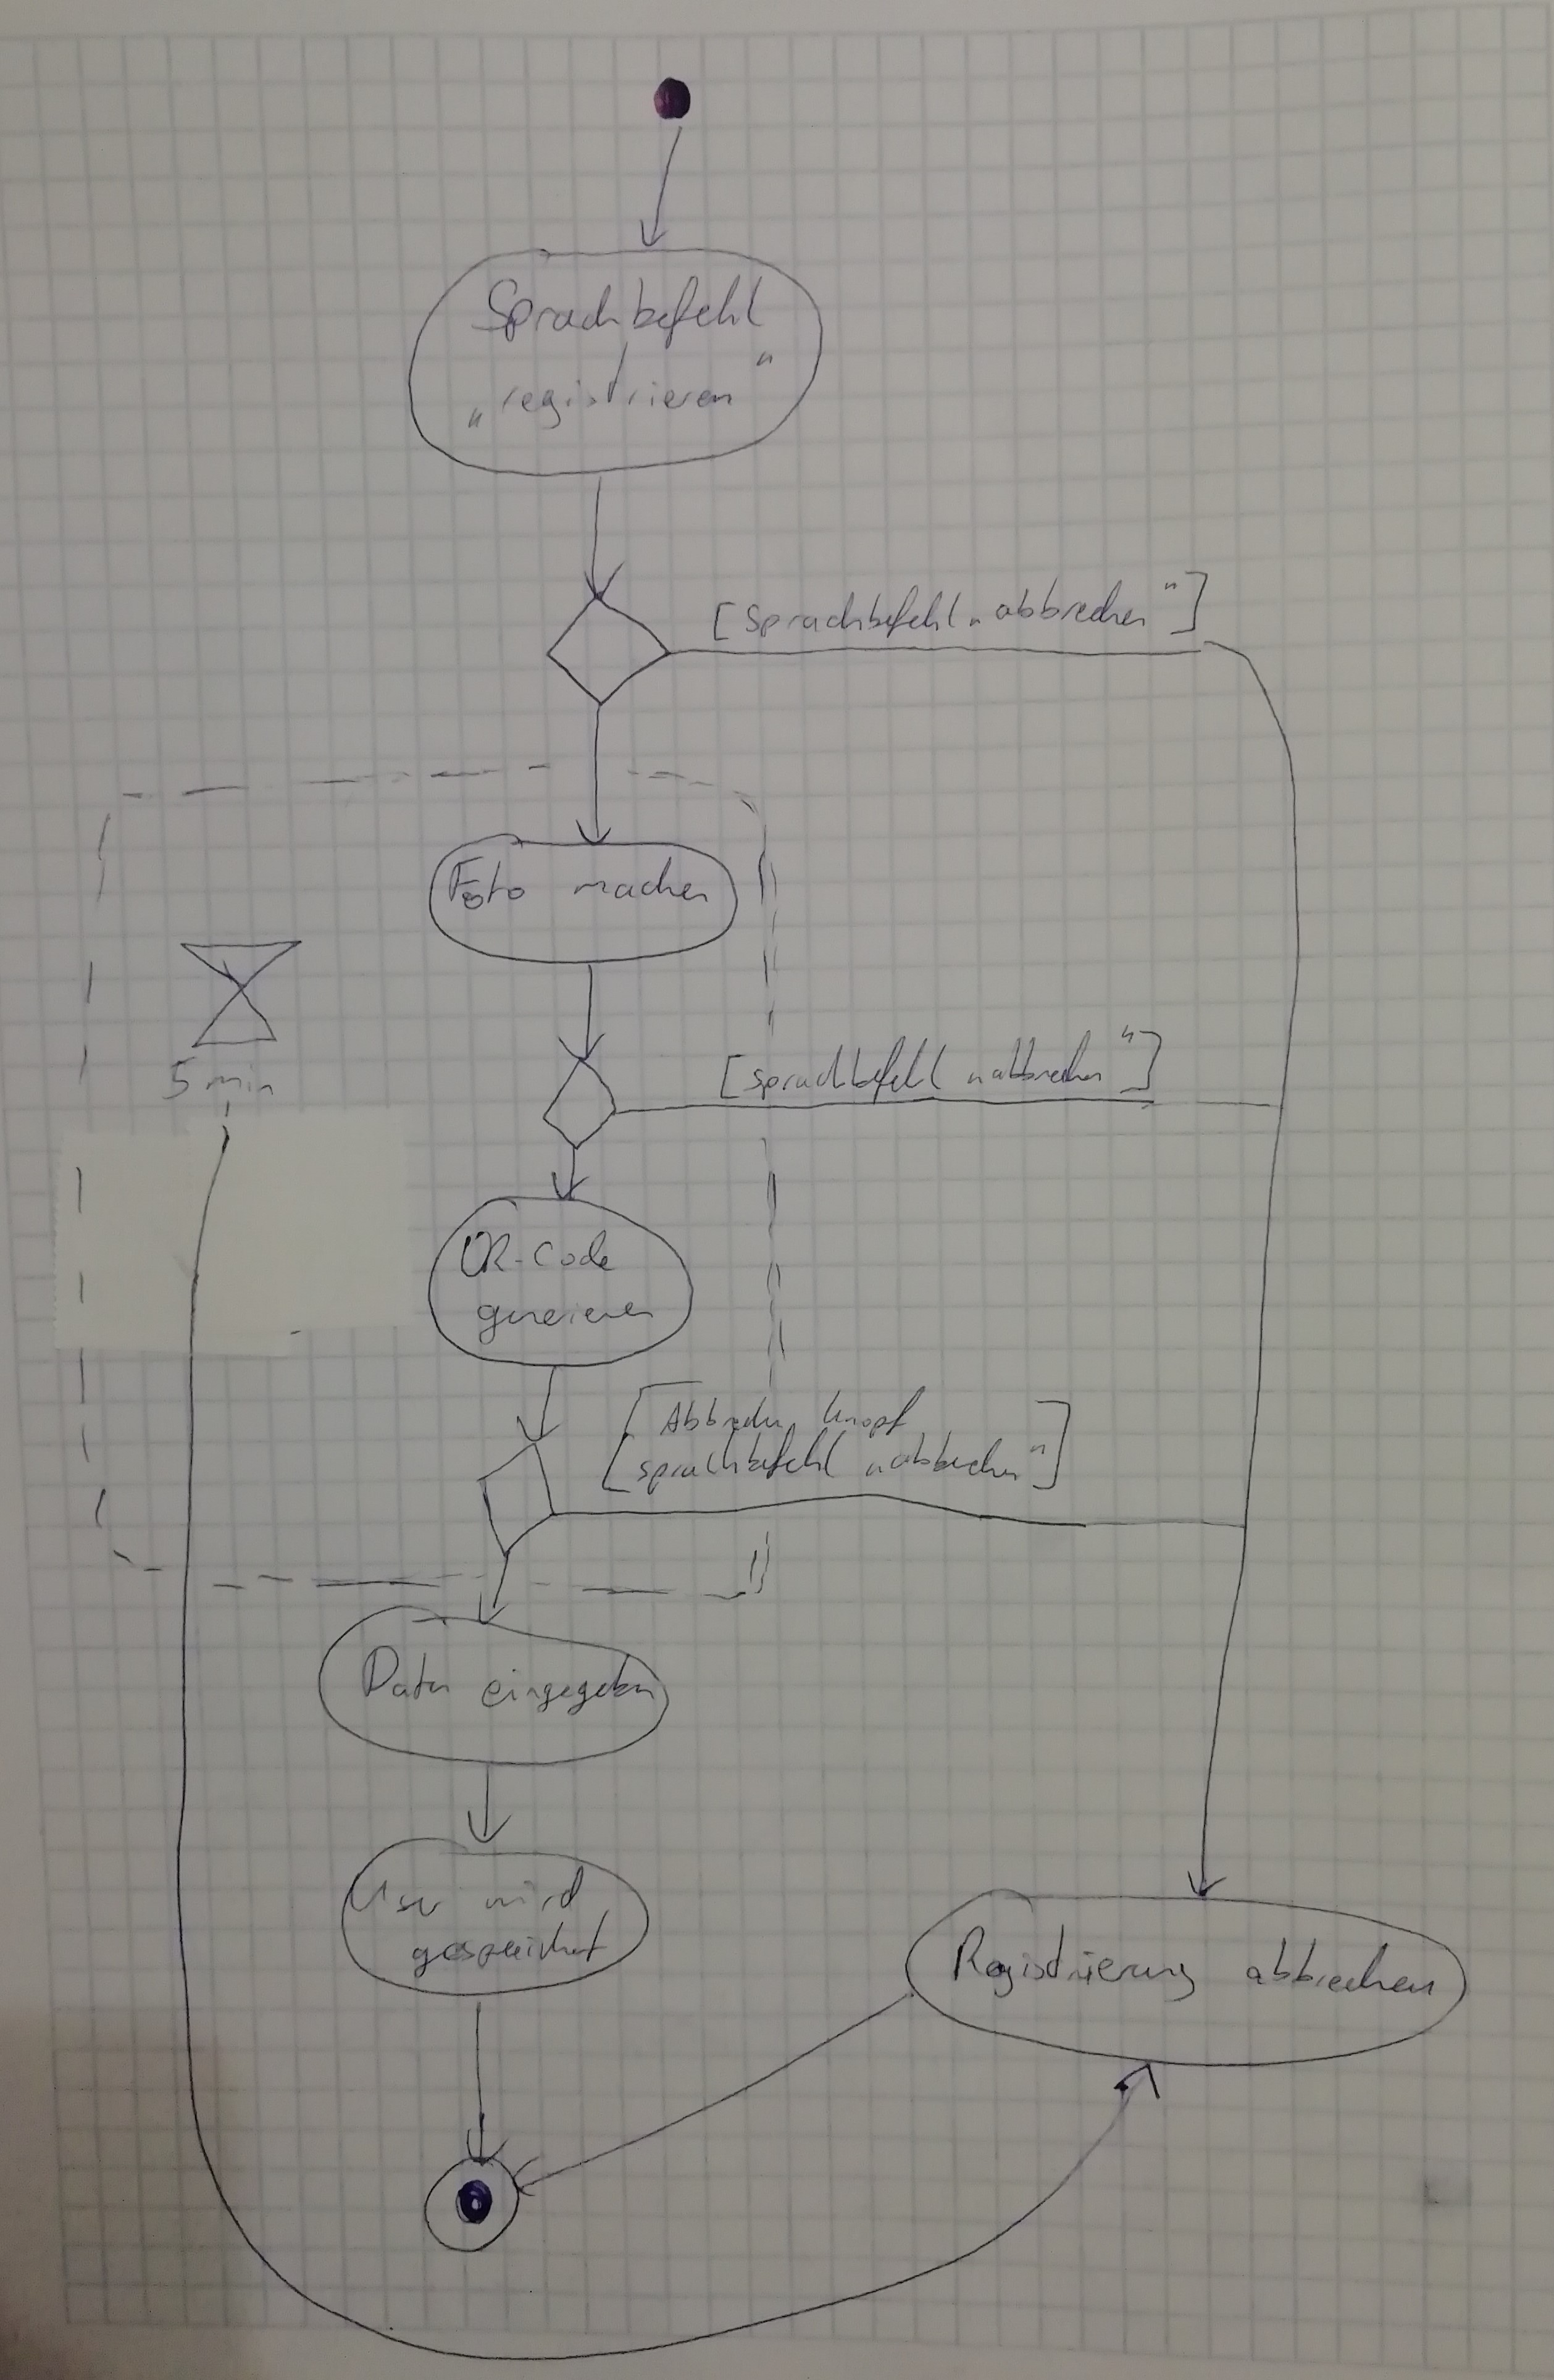
\includegraphics[scale=.17]{Activity.jpg}\\

\subsection{Use Case 10: Alternative to QR-Code}
\subsubsection{General Description}
\begin{tabular}{|p{.2\linewidth}|p{.65\linewidth}|}
\hline 
ID: & Alternative to QR-code\\ \hline
Goal: & Be able to register via the app without scanning a qr-code. \\ \hline
Precondition: & Registration has started.\\ \hline
Postcondition: &  The user has registered via the qr-code alternative.\\ \hline
Involved Users: & Role name: user \\ \hline
\end{tabular}

\subsubsection{The Standard Use}
During the registration process, the app has to get the information, which IP the IP of the mirror owns. It either can get acquired by scanning the QR-code or an alternative, which is still in search.

\subsubsection{The Non-Standard Use}
The Dahoam-Connect App is not connected to the same WiFi as the mirror.

\subsection{Use Case 11: Admin Account}
\subsubsection{General Description}

An admin is a user with more permissions than a normal user for example:
\begin{itemize}
    \item set smart home devices
    \item manage other users
\end{itemize}\\

\begin{tabular}{|p{.2\linewidth}|p{.65\linewidth}|}
\hline 
ID: & Admin account\\ \hline
Goal: & To have a user with more permissions to manage users and smart home devices.\\ \hline
Precondition: & No one is able to manage the users or install new smart home devices.\\ \hline
Postcondition: & A user that is able to manage everything exists. \\ \hline
Involved Users: & Role name: admin \\ \hline
\end{tabular}


\subsection{Use Case 12: Demo Mode}
\subsubsection{General Description}
The demo mode is used on fairs to display the functionality of the mirror. \\
\\
\begin{tabular}{|p{.2\linewidth}|p{.65\linewidth}|}
\hline 
ID: & Demo mode\\ \hline
Goal: & To have a different mode than the normal use of the mirror for showing features under harder conditions (loud noise, many people).\\ \hline
Postcondition: &  The functionality and all features are getting correctly showcased.\\ \hline
Involved Users: & Role name: user \\ \hline
\end{tabular}

\subsubsection{The Standard Use}
Start the demo mode on a fair so that the features can be presented to the audience.

\subsubsection{The Non-Standard Use}
The features are not working correctly (because of other conditions than for normal use, like loud noise and many people)



\subsection{Use Case 13: Kiosk Auto Start}
\subsubsection{General Description}
The raspberry pi 4 just has to be plugged in and the mirror boots automatically. \\

\begin{tabular}{|p{.2\linewidth}|p{.65\linewidth}|}
\hline 
ID: & Kiosk auto start\\ \hline
Goal: & Plug it in and everything is ready to go. \\ \hline
Precondition: & The mirror has to be installed in a room and has power. \\ \hline
Postcondition: &  The Raspberry Pi 4 has booted and started Dahoam automatically.\\ \hline
Involved Users: & Role name: user \\ \hline
\end{tabular}

\subsubsection{The Standard Use}
The raspberry pi boots and starts the mirror application without anything else to be done. Without kiosk the user would have to write the command to start the mirror themselves, open the browser on localhost and connect on the right port. But to be the able to do this, it would be necessary to connect a mouse, keyboard and screen to the  raspberry pi 4.

\subsubsection{The Non-Standard Use}
When the raspberry pi can not connect to the last used network or was never connected to any, it starts the network configuration in order to let the user connect it to an available network. 

\subsection{Use Case 14: Session Management}
\subsubsection{General Description}

User should be logged in and out as fast as possible. Also it should not be possible to use all commands  by a person that is not registered. 

\begin{tabular}{|p{.2\linewidth}|p{.65\linewidth}|}
\hline 
ID: & Session management\\ \hline
Goal: & Improve the session management for login and register and restrict some commands to logged in users.\\ \hline
Precondition: & Everyone can use all commands and it takes quit a long time to be logged in and out.\\ \hline
Postcondition: & Only authorised users can use the mirror to its full extent.\\ \hline
Involved Users: & Role name: user \\ \hline
\end{tabular}

\subsubsection{The Standard Use}
When a user is registered, all commands can be used.

\subsubsection{The Non-Standard Use}
In demo mode, commands are still available, even if no one is logged in.


\pagebreak

\section{Non-Functional Requirements}
\subsection{NFR 1: Enable Full Dockerized Runtime Environment}
\begin{tabular}{|p{.2\linewidth}|p{.65\linewidth}|}
\hline 
ID: & Full dockerized runtime environment \\ \hline
Name: & Enable full dockerized runtime environment \\ \hline
Type	: & USE\\ \hline
Description: & It is really complicated and takes a lot of time to install all required software and programming languages on the Raspberry Pi 4. Therefore, a Docker runtime environment should fix this.\\ \hline
\end{tabular}

\subsection{NFR 2: Development Environment}
\begin{tabular}{|p{.2\linewidth}|p{.65\linewidth}|}
\hline 
ID: & Development environment \\ \hline
Name: & Development environment \\ \hline
Type	: & MAINT\\ \hline
Description: & Instead of always compiling or running the whole project, a development environment gets offered for developer, so different parts of the project can be build and tested independent of each other.\\ \hline
\end{tabular}

\subsection{NFR 2.1: Isolated Testing with Node-RED}
\begin{tabular}{|p{.2\linewidth}|p{.65\linewidth}|}
\hline 
ID: & Isolated testing with node-RED \\ \hline
Name: & Isolated testing with node-RED \\ \hline
Type	: & USE\\ \hline
Description: &  Developers will be able to test different sections of the mirror like the speech or masterservice separately from each other. There are different test cases prepared on node-RED so that testing is easier. This will improve the time it takes to test single components and identify the exact location of bugs and errors. \\ \hline
\end{tabular}

\subsection{NFR 2.2: Improved logging}
\begin{tabular}{|p{.2\linewidth}|p{.65\linewidth}|}
\hline
ID: & Improved logging \\ \hline
Name: & Improved logging \\ \hline
Type	: & USE\\ \hline
Description: &  Each component will log data in a separated log file, which will make finding problems easier. The developer shall also be able to change the log level of each component, so that only the important information for their specific problem are logged.\\ \hline
\end{tabular}

\subsection{NFR 3: 24/7 Runtime Performance}
\begin{tabular}{|p{.2\linewidth}|p{.65\linewidth}|}
\hline 
ID: & 24/7 runtime performance \\ \hline
Name: & 24/7 runtime performance \\ \hline
Type	: & EFFIC\\ \hline
Description: & Programs that run for a long time have to cope with memory leaks and docker container that get unhealthy. Therefore, a technique has to be developed that is able to cope with those kind of problems.\\ \hline
\end{tabular}

\subsection{NFR 4: Profile Picture}
\begin{tabular}{|p{.2\linewidth}|p{.65\linewidth}|}
\hline 
ID: & Profile picture \\ \hline
Name: & Profile picture \\ \hline
Type	: & USE\\ \hline
Description: & The picture that was taken while registration will be shown to the user. The user is also able retake this picture.\\ \hline
\end{tabular}

\subsection{NFR 5: Encrypt User Password before Storing in the Database}
\begin{tabular}{|p{.2\linewidth}|p{.65\linewidth}|}
\hline 
ID: & Encrypt user password before storing in the database \\ \hline
Name: & Encrypt user password before storing in the database \\ \hline
Type	: & SEC\\ \hline
Description: & For a higher security the password has to be encrypted or at least stored as a hash code. \\ \hline
\end{tabular}


\subsection{NFR 6: Improve Speech Recognition Quality}
\begin{tabular}{|p{.2\linewidth}|p{.65\linewidth}|}
\hline 
ID: & Improve speech recognition quality \\ \hline
Name: & Improve speech recognition quality \\ \hline
Type	: & EFFIC\\ \hline
Description: & The speech recognition sometimes does not understand the spoken words correctly. If there is a lot of background noise, this problem gets worse and worse. In order to achieve best perform this problem has to be fixed.\\ \hline
\end{tabular}

\subsection{NFR 7: Dahoam-Flaws}
\begin{tabular}{|p{.2\linewidth}|p{.65\linewidth}|}
\hline 
ID: & Dahoam-Flaws \\ \hline
Name: & Dahoam-Flaws \\ \hline
Type	: & USE\\ \hline
Description: & When speaking to the mirror it often understands wrong things. E.g.: ``Schalte das Licht in Raum 2 und 3 ein'' then it adds the two numbers and turns on the light in room 5. Furthermore a problem occurs when several registered users are in front of the mirror because it can not decide which of them should be logged in. When an unregistered user kicks off registration process and denies it, the whole registration process is blocked for the running session.\\ & 
While registration, a live camera feedback should help the user positioning himself in the right place. This prevents bad profile pictures.
\\ \hline
\end{tabular}


\pagebreak

\section{Quantity Structure}

Because of high data processing, the Raspberry Pi 4 gets very hot. That's caused by incoming voice data and camera feedback.

\pagebreak
\section{System Architecture and Interfaces}
Dahoam is embedded either in a common home without any smart home interfaces or in a modern home with some smart home lights or sensors installed.\\
The user is able to communicate with the mirror either with speech recognition or Dahoam-Connect-App. \\
The mirror has a connection to a weather API and has an interface to get the emails of the user via IMAP. It is also capable of addressing the calendar which is saved on the phone of the user. \\


\pagebreak
\section{Acceptance Criteria}
\subsection{Delete User}
If a user is deleted, all related data must be removed. If a user removes their account through Dahoam-Connect-App, a confirmation message appears and the user will be redirected to the login view. If they are meanwhile logged into the mirror, they should be logged out after the deletion process. \\
\newline
\textbf{First Configuration of the Mirror}\\
The configuration must include:
\begin{itemize}
    \item Create an admin account for all further configurations
    \item Connect to an existing network (on-/offline does not matter) in order to communicate with Dahoam-Connect-App
    \begin{itemize}
        \item Online: Enter location for the weather display
    \end{itemize} 
\end{itemize}
\subsection{First Configuration of the Mirror}
The mirror has to be able to connect to a WiFi via a website on their smart phone.
\subsection{Install Smart Home Interfaces}
For configuration of smart home devices, an own page in Dahoam-Connect-App is required. Following information is required:
\begin{itemize}
    \item MQTT-Broker IP and port
    \item A username and password if needed
    \item Publish
    \begin{itemize}
        \item Name
        \item Topic
        \item QoS and retained
        \item Values
    \end{itemize}
    \item Subscription
    \begin{itemize}
        \item Name
        \item Topic
        \item QoS
    \end{itemize}
\end{itemize}
\\
After entering the required information the data from the smart home device should be received correctly.
\subsection{User Administration}
The admin has to be able to delete other accounts and giving them admin rights. An admin is also capable of seeing all other accounts.
\subsection{Sleep Mode}
The mirror is able to go into sleep mode and save power by doing so.
\subsection{Wake up from Sleep Mode}
When the motion sensor detects movement, the mirror starts the face recognition and checks if a registered user stands in front of it. 
\subsection{Creating First Admin}
While first registration process, the first user will automatically be set as an admin.
\subsection{Defining Personal Location}
The user is capable of defining an own location to be shown at the mirror screen instead of seeing the mirrors default location.
\subsection{Registration Flow}
The user starts the registration flow with a spoken command and can also abort it by a timeout or by a speech command or pressing the ``abbrechen'' button in the Dahoam-Connect App. 
\subsection{Alternative to QR-Code}
An alternative to QR-code exists to connect the Dahoam-Connect App with the mirror.
\subsection{Admin Account}
The admin should be able to delete other users, install smart home devices and configure the default mirror weather location
\subsection{Demo Mode}
At a fair the mirror can be presented without any problems and all features can be showcased to the audience.
\subsection{Kiosk Auto Start}
When plugging in the mirror the setup and starting of the application is done automatically.
\subsection{Session Management}
The mirror logs out the user automatically, when the interaction between user and mirror stops.
\end{document}  